Im folgenden Kapitel werdenBevor in die Arbeit eingestiegen werden kann, müssen zunächst einige Begriffe geklärt, die Ausgangssituation dargestellt und das Thema etwas abgesteckt werden.

\section{Begriffe}
\subsubsection{App/Applikation/Anwendung}
Im Rahmen dieser Arbeit wird oft von einer App oder Applikation geredet. Damit ist eine Anwendung gemeint, die für mobile Endgeräte entwickelt wurden. Die am häufigsten genutzten mobilen Geräte sind dabei Smartphones mit einem Marktanteil von etwa 62,6\%\footnote{https://gs.statcounter.com/os-market-share}.

\subsubsection{Plattform}
Der Begriff Plattform kann auf unterschiedliche Betriebssysteme, Prozessortypen, Kommunikationsprotokolle oder Hardwaresysteme bezogen werden \cite{2014Mulit_plattform_definition}. In dieser Arbeit werden damit die unterschiedlichen Betriebssysteme bezeichnet. Beispiele für diese sind Android, iOS oder auch MacOS.

\subsubsection{Multi-Plattform-Anwendung}
Als Multi-Plattform-Anwendung werden jene Anwendung bezeichnet, die auf mehreren Plattformen ausgeführt werden kann und dabei eine gleiche oder ähnliche Funktionalität hat \cite{2014Mulit_plattform_definition}. Eine Anwendung muss dabei nicht für alle Plattformen implementiert sein. Ist eine Anwendung auf mehr als einer Plattform verfügbar so kann diese als Multi-Plattform-Anwendung bezeichnet werden.

\subsubsection{Cross-Plattform-Anwendung}
Cross-Plattform-Anwendungen sind ebenfalls, wie Multi-Plattform Anwendungen, auf mehr als einer Plattform ausführbar. Der Unterschied besteht darin, dass Cross-Plattform-Anwendungen eine gemeinsame Codebasis besitzen, die es ermöglicht, die Applikation nur einmalig implementieren zu müssen, jedoch mehrere Plattformen damit abdecken zu können \cite{2014_Cross_plattform}.

\subsubsection{GraphQL}
GraphQL\footnote{https://graphql.org/} ist eine von Facebook vorgestellte Schnittstellen-Technologie für Web-Server. Im Gegensatz zur oft genutzten REST-API kann der Client dabei die Struktur und den Aufbau der Antwort festlegen, wodurch das Senden von unnötigen Daten verhindert wird. Die Kommunikation findet dabei mit Hilfe von JSON statt. Eine Untersuchung von Brito et al \cite{IEEE_GraphQL} ergab, dass durch die Verwendung von GraphQL eine Reduktion der gesendeten Datenmenge um bis zu 99\% erreicht werden kann. 

\section{Unterschiedliche Ansätze der Applikationsentwicklung für mobile Engeräte}
\label{cha:3_2}
Für die Programmierung von Multi-Plattform Applikationen gibt es unterschiedliche Ansätze, in die die Entwicklungsmethoden eingeordnet werden können. Dabei unterscheiden verschiedene Autoren unterschiedliche Ansätze. In dieser Arbeit wird dafür die von Delia et al \cite{IEEE_development_classes} definierten Einteilung verwendet. Im Folgenden werden diese vorgestellt sowie einzelne Aspekte betrachtet.

\subsection{Native Applikationen}
Native Applikationen werden entwickelt, um auf einer einzelnen Plattform eingesetzt zu werden. Der Quellcode wird dafür in ausführbaren Code übersetzt. Dieser ist spezifisch für die gewählte Plattform \cite{IEEE_development_classes}.
Die Programmierung wird in der plattform-typischen Programmiersprache geschrieben und ist dadurch nur für eine Plattform nutzbar. Es gibt folglich für jede Plattform einen eigenen Quellcode. Um etwa eine native Android App zu entwickeln, wird diese in Kotlin programmiert und im Anschluss in Kotlin-Bytecode übersetzt. Dieser Bytecode ist dabei lediglich auf Android Geräten ausführbar.

Ein Vorteil der nativen Entwicklung ist, dass die Funktionen der verschiedenen Plattform optimal genutzt werden können. Die von den Geräten zur Verfügung gestellten Schnittstellen müssen dabei lediglich aufgerufen werden. So können beispielsweise Kamera, GPS oder auch Kalender einfach und effizient genutzt werden. Dabei ist die Ausführung nicht nur performant, sondern kann auch unkompliziert in einem Hintergrundprozess gestartet werden \cite{IEEE_development_classes}.
Zusätzlich stellen die Plattformen UI-Elemente für die native Entwicklung zur Verfügung, so dass das Aussehen der Applikation und der Benutzerschnittstellen ähnlich zu der unterstützten Plattform ist. So entsteht für den Nutzer ein geschlossenes System, das leichter zu bedienen ist, da es kaum Unterschiede in Struktur, Design, Aufbau oder auch Benutzung gibt \cite{IEEE_Khackouch_Al}.

Ein Nachteil der nativen Entwicklung von Multi-Plattform Anwendungen ist der Aufwand und die damit verbundenen Kosten. Da die Anwendung für jede Plattform einzeln verwirklicht werden muss. So können die Gesamtkosten durch die Multiplikation der Entwicklungskosten einer Plattform mit der Anzahl der zu unterstütztenden Plattformen geschätzt werden \cite{IEEE_Khackouch_Al}. Doch nicht nur die initiale Implementierung ist kostenintensiv. So nennen Delia et al \cite{IEEE_development_classes} auch das Testen, Abändern und Verteilen neuer Versionen als Kosten, die auf jeder unterstützten Plattform auftreten. 
Um die Kosten zu verringern, können deswegen anfänglich einzelne Plattformen zur Implementierung ausgewählt werden, wodurch jedoch die Zahl der potentiellen Nutzer sinkt.

\subsection{Web-Applikationen}
\label{cha:3_2_web}
Web-Applikationen sind Applikationen, die im Internet verfügbar sind. Sie sind darauf ausgelegt, als Webanwendungen auf einem Server zu laufen und dann mittels eines Browser auf dem Geräte aufgerufen zu werden. Der Nutzer kann ohne zusätzliche Installation die Anwendung nutzen, sobald der Server gestartet wurde \cite{IEEE_Khackouch_Al}.
Da sie auf allen Geräten mit einem Browser und einer Internetverbindung aufgerufen werden kann, müssen keine plattformspezisfischen Versionen entwickelt werden.
So können alle Plattformen mit nur einer Entwicklung abgedeckt werden \cite{IEEE_development_classes}.

Wie bereits erwähnt, können Entwicklungskosten gesparrt werden, da nur ein Code für alle Plattformen geschrieben wird. Ein weiterer Vorteil ist, dass Updates dem Nutzer direkt nach einem Neustart des Servers zur Verfügung stehen, da diese nicht erst an die Geräte verteilt und dann installiert werden müssen \cite{IEEE_Khackouch_Al}. Des Weiteren können mittlerweile selbst Laien Webseiten erstellen, da Firmen wie beispielsweise Squarespace\footnote{\url{https://de.squarespace.com/}} die Erstellung stark vereinfacht. So muss gerade einmal eine Vorlage ausgewählt werden und das Design auf das Projekt angepasst werden, um eine nutzbare Webanwendung zu erhalten. 
Außerdem kann der Code einer Webapplikation wiederverwendet werden, um etwa eine hybride Applikation, wie sie im Kapitel \ref{cha:3_hybrid} erklärt wird, zu erstellen \cite{IEEE_Khackouch_Al}. 

Jedoch ist die nutzbare Funktionalität der Plattform, durch die Beschränkungen des genutzten Browsers limitiert. Dabei können lediglich die Funktionalitäten genutzt werden, auf welche der Browser Zugriff hat \cite{Phyo}. Hinzukommend tritt bei einer langsamen Internetverbindung eine erhöhte Ladezeit auf und infolge dessen sinkt die Performance. Wenn eine Internetverbindung gänzlich nicht verfügbar ist, kann die Anwendung gar nicht genutzt werden \cite{IEEE_Khackouch_Al}. Des Weiteren müssen Webanwendungen zur Nutzung auf Smartphones angepasst werden, um auf unterschiedliche Seitenverhältnisse und Auflösungen reagieren zu können. So sind Smartphones etwa höher als breit und haben daher weniger Platz in der Menüleiste als etwa bei einer Nutzung an einem Computer. Folglich muss abhängig der Bildschirmauflösung ein angepasstes Design zur Verfügung gestellt werden \cite{Serrano_mobile}.

Web-Applikationen sind in den letzten Jahren, durch die Verfügbarkeit von schnellen Internetverbindungen in fast allen Teilen der Welt, einfacher nutzbar geworden.
Im Schnitt stieg die mobile Bandbreite zwischen 2017 und 2021 um 59,5\% beziehungsweise von knapp 20 Mbps auf 55 Mbps\footnote{\url{https://www.ookla.com/articles/global-index-2019-internet-report}}.
Jedoch ergab eine Studie\cite{report_webusage} von Yoram Wurmser, dass während der Nutzung des Smartphones, amerikanische Erwachsene etwa 89\% der Zeit in Applikationen und gerade einmal 11\% in einem Browser verbringen.

\subsection{Hybride Applikationen}
\label{cha:3_hybrid}
Der Ansatz der Entwicklung einer hybriden Applikation teilt viele Eigenschaften mit den Web-Applikationen.
Sie nutzen Web-Technologien, wie beispielsweise HTML, Javascript und CSS, werden jedoch in einer Applikation mit einem Webcontainer und nicht im Browser des Geräts ausgeführt \cite{IEEE_development_classes}.
Die hybride Applikation verfügt hierbei über eine Schnittstelle, mittels welcher sie Zugriff auf die Funktionalität der Plattform erhält.

\begin{figure}[ht]
  \centering
  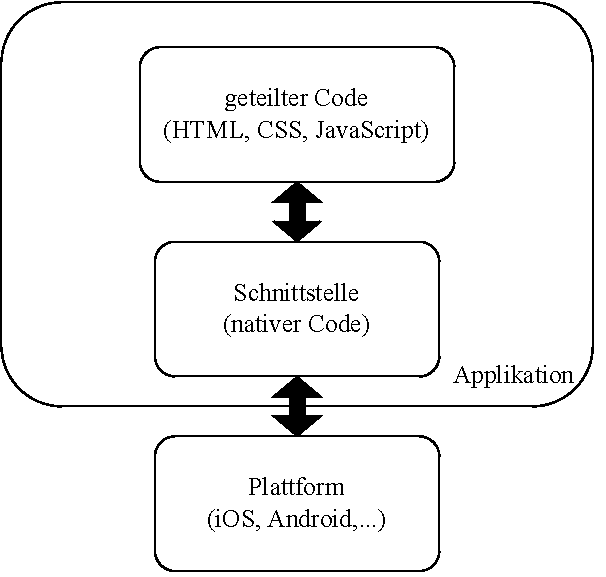
\includegraphics[height=9cm,keepaspectratio]{images/hybrid_architecture.drawio.pdf} 
  \caption{Architektur einer hybriden Applikationen}
  \label{fig:hybrid_architecture}
\end{figure}

Wie in Abbildung \ref{fig:hybrid_architecture} zu sehen ist, besteht diese Art von Applikation aus zwei Teilen.
Der erste Teil ist ein geteilter Code, der mit Web-Technologien erstellt wird und sowohl die UI als auch Applikationslogik enthält. Der geteilte Code kann dabei sowohl lokal als auch auf einem Server gespeichert werden und ist für mehrere Plattformen verwendbar \cite{2017hybrid_approach_end}.
Der zweite Teil formt eine Schnittstelle, die in nativen plattformspezifischen Code geschrieben ist. Der Schnittstellencode kann entweder selbstständig implementiert werden oder von einem Schnittstellen-Framework wie Cordova\footnote{\url{https://cordova.apache.org/}} zur Verfügung gestellt werden. Die Schnittstelle verwirklicht eine bidirektionale Kommunikation zwischen der Plattform und der Applikationslogik \cite{ELKASSAS2017163}. Somit kann die Anwendung auf die Funktionalitäten der Plattform zugreifen. Zusätzlich ermöglicht sie die Darstellung der Anwendung auf dem Endgerät. 

Grundsätzlich teilt dieser Ansatz die gleichen Vor- und Nachteile wie Web-Applikationen, da er zu einem großen Teil die selbe Technologien nutzt. Jedoch kann eine offline Funktionalität erreicht werden, wenn die Anwendung lokal gespeichert ist. Zusätzlich erhält die Applikation durch die Schnittstelle Zugriff auf die native Funktionalität und kann auf dem Gerät installiert werden. Weiterhin kann der geteilte Code sowohl auf den verschiedenen Plattformen, als auch in anderen Technologien wiederverwendet werden, da es sich im Prinzip um eine Webseite innerhalb einer Applikation handelt \cite{IEEE_development_classes}. Jedoch entsteht durch den zusätzlichen Web-Container, der geladen werden muss, um die UI anzuzeigen, eine erhöhte Ladezeit, die sich negativ auf die Performance der Applikation auswirkt \cite{IEEE_development_classes}.

\subsection{Interpretierte Applikationen}
\label{cha:3_2_interpretiert}
Bei interpretieren Cross-Plattform Anwendungen schreibt der Entwickler Code, der anschließend mithilfe eines Interpreters während der Laufzeit in ausführbaren Code übersetzt wird. Folglich besteht die auf dem Gerät installierte Anwendung aus zwei Teilen. Einerseits einem nativen Teil, oftmals Frameworkcode, der zum Übersetzen der eigentlichen Anwendung benötigt wird. Andererseits einem Cross-Plattform Teil, der die Anwendungslogik realisiert \cite{IEEE_development_classes}.

Der Unterschied zu einer hybriden Applikation besteht darin, dass die Anwendungen je nach Plattform anders aussehen können. So wird etwa die Benutzeroberfläche erst während der Laufzeit in eine native UI, mit den plattformspezifischen UI Elementen, übersetzt.
Dadurch wird eine Nutzung von nativen Elementen möglich, obwohl die Anwendung eigentlich in einer anderen Sprache definiert ist \cite{IEEE_development_classes}. 
Dazu kommt, dass eine Anwendungen auf allen Plattformen ausgeführt werden kann, die von dem entsprechenden Interpreter unterstützt wird \cite{server_side}.

Jedoch ergibt sich hierbei eine Abhängigkeit zum Framework und dessen unterstützten Plattformen. Zudem hat, durch die Interpretierung während der Laufzeit, dieser Ansatz eine hohe Reaktionszeit, da jede Zeile vor Ausführung erst durch den Interpreter übersetzt werden muss und somit eine extra Latenz zwischen jedem einzelnen Aufruf und dessen Ausführung entsteht \cite{server_side}.

\subsection{Cross-kompilierte Applikationen}
Bei cross-kompilierten Applikationen wird während der Entwicklung ebenfalls lediglich ein Quellcode geschrieben, jedoch wird dieser bereits vor Verteilung in nativen Code übersetzt. Daher muss der Übersetzungsprozess nur einmalig durchgeführt werden und nicht wie bei dem interpretierten Ansatz, bei jeder Benutzung. Um dies zu erreichen, wird ein Cross-Compiler benötigt, der für mehrere unterschiedliche Plattformen Kompilate erzeugt \cite{mobiledraft_cross_plattform}. Somit kann aus einem Code für jede Plattform eine eigene Anwendung gebaut werden, die ausschließlich aus nativem Code besteht und sich folglich für das Betriebssystem nicht von einer nativen Anwendung unterscheidet \cite{IEEE_development_classes}.Im Vergleich zur interpretieren Anwendung kann außerdem die App-Größe reduziert werden, da kein zusätzlicher Übersetzer benötigt wird \cite{mobiledraft_cross_plattform}.

Auch bei diesem Ansatz ist die Funktionalität und die Zahl der unterstützten Plattformen von dem genutzten Cross-Compiler abhängig. Einige dieser Frameworks nutzen eine spezialisierte Programmiersprache, sodass eine Wiederverwendung des Codes für einen anderen Ansatz erschwert wird. So wird etwa bei Flutter\footnote{\url{https://flutter.dev/}} die Sprache Dart\footnote{\url{https://dart.dev/}} genutzt.

\subsection{Gemischter Ansatz}
Die Entwicklungsansätze sollen in dieser Arbeit um einen weiteren Ansatz erweitert werden, wie ihn Khachouch et al \cite{IEEE_Khackouch_Al} in ihrer Arbeit aufführen. Sie definieren einen gemischten Ansatz, um die verschiedenen Ansätze kombinieren zu können. Somit können die Vorteile unterschiedlicher Ansätze vereint werden.


\section{Themenabgrenzung}
In dieser Arbeit sollen nicht die verschiedenen Programmiersprachen oder Frameworks innerhalb der einzelnen Ansätze verglichen werden, sondern viel mehr die Ansätze gegenseitig. Daher wird für eine Cross-Plattform Implementierung das Framework Flutter\footnote{https://flutter.dev/} genutzt, da dies das aktuell am meisten genutzte Framework\cite{statist_CP_Framework} ist und somit einen guten Repräsentanten für diese Gruppe darstellt. Für die Android Implementierungen wurde als Programmiersprache Kotlin\footnote{https://kotlinlang.org/} genutzt. 

Die nativen Implementierungen werden in dieser Arbeit auf eine Android Implementierung beschränkt. 
Einerseits sind iOS und Android vergleichbar, da beide nativ auf die vollständigen Funktionalitäten der Betriebssysteme zugreifen.
Dabei sind es nicht die verschiedenen Programmiersprachen und ihre Kleinigkeiten die entscheidend sind, um native Apps zu entwickeln, sondern die Konzepte.
So sagen Goadrich et al \cite{iOSvsAndroid} in einer Untersuchung, welche Plattform für einen Universitätskurs passend wäre, dass beide Umgebungen die für den Kurs benötigten Funktionalität haben.
Weiter sagen sie, dass Studenten dadurch praktische Erfahrung in der Applikationsentwicklung bekommen würden. Sie kommen am Ende auf den Schluss, dass es kein Unterschied macht welche Plattform dabei behandelt werden würde und beide Plattformen helfen, eine Grundlage zur Lehre der Grundideen für mobile Endgeräte Programmierung bilden würden.
Auch in Sachen Performance gibt es zwischen den Plattformen keine größere Unterschiede. So zeigt eine Untersuchung von Győrödi et al \cite{Android_IOS_Performance_comparison}, dass es zwar kleinere Unterschiede in der Performance gibt, es aber keine Plattform gibt, die insgesamt gesehen besser ist, als die andere.
Desweiteren stellt Android die deutlich größere Nutzergruppe dar. So besagen aktuelle Statistiken, dass Android aktuell einen Marktanteil von etwa 70\% hat, während iOS nur auf 30\% kommt \cite{statist_OS_worldwide}.  

Die betrachteten Implementierungen umfassen ebenfalls keine Spieleimplementierung. Diese stellen zwar einen signifikanten Teil der in den Appstores vorhandenen Anwendungen dar, jedoch sind dies keine typischen Apps die von Appagenturen oder privaten Entwicklern produziert werden, sondern eher von Unternehmen mit Grafik- oder Spieleentwicklungshintergrund. Außerdem werden die meisten Apps nicht in Kotlin oder Swift direkt entwickelt, sondern mit Game- und Grafikprogrammen wie Unity oder ähnlichem gebaut. 



Der Schwerpunkt der Arbeit liegt außerdem auf Smartphone-Applikationen. Zwar sind in der Klasse der mobilen Endgeräte auch Laptops mit den Betriebssystemen Windows, MacOS oder die verschiedenen Linux distributionen, dennoch werden Applikationen primär für den Smartphone Markt entwickelt, während für mobile Rechner dann eher ein Programm schreibt.
\TODO{Warum auf Smartphone bei Untersuchung beschränkt?}


%\section{Projektbeschreibung}
Als Basis für diese Arbeit wird eine bereits bestehende Elixir-Web-Anwendung genutzt. Hierbei handelt  es sich um eine Plattform, die das Ziel hat, das Verleihen und Leihen innerhalb von Bekanntschaftskreisen zu vereinfachen/ ermöglichen. Hierfür kann jeder Nutzer seine eigenen, verleihbaren Gegenstände auf der Plattform eintragen. Zusätzlich können Nutzer sogenannte Kreise erstellen und zusammen mit Freunden bzw. Familie beitreten. Jeder kann dann die Gegenstände sehen, die in den verschiedenen Kreisen vorhanden sind, in denen er Mitglied ist. Zur Kontaktaufnahme gibt es ein Chatsystem, bei dem sich Leute Nachrichten hin und her schicken können, um den Austausch zu organisieren. Zur Kommunikation mit einer Applikation besitzt das System eine GraphQL-Schnittstelle, über die alle benötigten Daten abgefragt werden können. Auch kann der Nutzer über die Schnittstelle authentifiziert werden und neue Nachrichten versendet.

\section{Funktionsumfang der Beispiel-Anwendung}
Damit die abgebildete Anwendung ein gutes Beispiel für eine Applikationsentwicklung darstellt, wurde beim Entwurf des Funktionsumfangs darauf geachtet, möglichst viele der typischen Funktionalitäten von Applikationen abzudecken. Eine Befragung \cite{JetBrains_miscellaneous_2021} mobiler Anwendungsentwickler durch JetBrains ergab, dass die wichtigsten Funktionen Datenspeicherung, Kommunikation über Netzwerk, Medienanzeige, Statusmanagement, Navigation, Datensynchronisierung, Dateien lesen/schreiben sind.
Das in der Arbeit betrachtete Projekt beschränkt sich dabei auf folgende Funktionalitäten:

Es soll eine App gebaut werden, die sich an der bestehende Web-Anwendung orientiert und einen Teil der Funktionalität durch die Programmierung abbildet. Dabei können die Implementierungen in zwei Gruppen unterteilt werden, die im Folgenden genauer beschrieben werden.

\subsubsection{Funktionalität mit Applikationscode}
Bei der nativen und der cross-kompilierten Applikation wird die komplette Funktionalität innerhalb der implementierten Applikation abgebildet. Die Verbindungen zwischen den umgesetzten Benutzeroberflächen ist in Abbildung \ref{fig:pageflow} dargestellt. Dabei sind Pfeile mit flacher Spitze Weiterleitungen die automatisch passieren und Pfeile ohne eine Beschriftung Abläufe, die durch das Drücken eines Buttons implementiert sind. Außerdem entsprechen die Zustände in der Abbildung den einzelnen Seiten der Anwendung. Diese sind eine Start-, Login-, Profil-, Kommunikations- und eine Chatseite. Dadurch können die oben genannte Aspekte vollständig abgedeckt werden. So ist etwa durch den Login das Statusmanagment und die Kommunikation über ein Netzwerk implementiert. 

\begin{figure}[ht]
  \centering
  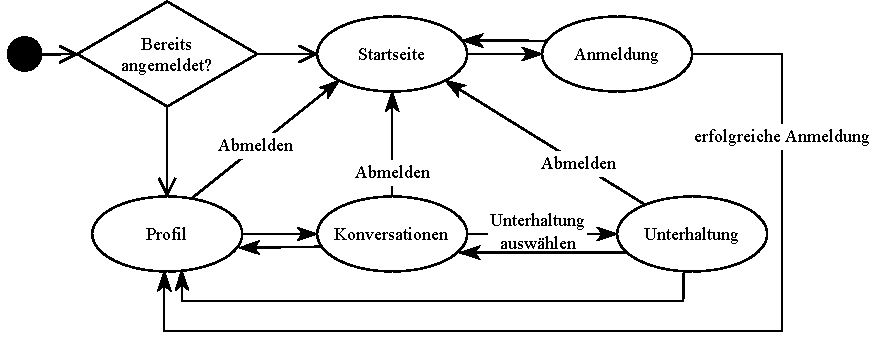
\includegraphics[height=7cm,keepaspectratio]{images/Pageflow_native_flutter.drawio.pdf} 
  \caption[Seitenablauf der implemierten nativen und cross-kompilierten Applikation]{Verbindungen zwischen den Seiten der implementierten Applikation des nativen und des cross-kompilierten Ansatzes}
  \label{fig:pageflow}
\end{figure}

Der Nutzer verwendet die Anwendung, wie im Folgenden beschrieben. Zunächst wird die App geöffnet. Wenn der Nutzer nicht eingeloggt ist, landet er auf einer Startseite/Willkommensseite, von welcher aus er sich einloggen kann. Ist er jedoch angemeldet, so wird er automatisch auf die Profil Seite weitergeleitet, auf der von einem Server geladene Daten angezeigt werden. Er kann außerdem auf das integrierte Chatsystem zugreifen und auch neue Nachrichten an andere Nutzer verschicken. Von allen Seiten mit benötigter Authentifizierung, gelangt der Nutzer durch Abmelden wieder auf die Startseite.

\subsubsection{Funktionalität mit Web-Integrierung}
In dieser Gruppe wird ein Teil oder auch die komplette Applikationslogik durch das Einbinden der Web-Anwendung in die Applikation ersetzt. So wird bei der Implementierung des hybriden Ansatzes die bereits existierende Website in eine native programmierte Applikation eingebunden. Der Applikationscode übernimmt dabei die Aufgaben, die klassischer Weise durch ein Framework erfüllt werden würde. Sie ist jedoch durch die spezifische Implementierung der Webseite stark in der Funktionalität eingeschränkt.

Bei der gemischten   Implementierung wird zwischen der Web-Anwendung und Benutzeroberflächen, die mit dem Cross-Compiler Framework Flutter erstellt wurden, gewechselt. Dabei werden insbesondere der Login, die Profilseite und das Chat System durch Flutter Seiten ersetzt, während der Rest der Anwendung durch die Web-Anwendung dargestellt wird. Daher ist dieser Ansatz eine Mischung aus dem hybriden und dem cross-kompilierten Ansatz.


